\section{Introduction}
    \label{sec:intro}
    Semantic 3D segmentation using U-Net models has become an integral part of a huge variety of medical image analysis pipelines, including registration, image-guidance, localisation and diagnostics. The nnUNet framework \cite{isensee2021nnu} has set new state-of-the-art accuracies in most recent benchmarks due to its potent parameterisation, rule-based architecture recommendation and robust pre-processing and augmentation. It comes at the cost of very large models and extensive test-time augmentations that may limit an efficient application in resource-limited environments among others in point-of-care healthcare or developing countries.

    \subsection{Related Work}
        A great number of complementary approaches exist that aim at limiting the kernels of deep convolutional networks, e.g. by constraining their quantisation \cite{zhang2021medq}, reducing their rank \cite{jaderberg2014speeding} or requiring symmetry \cite{marcos2016learning}. While translational-invariance is given for fully-convolutional architecture, equivariance against rotations has to be incorporated at the additional computational expense by augmentation strategies in training and at inference time. A particular popular direction of research explores the use of rotation equivariant networks \cite{cohen2016group} that employ multiple rotated versions of filters \cite{bekkers2018roto,dieleman2016exploiting} (or steerable filters \cite{weiler20183d}) and find a maximum response among them. While steerable 3D filters can have great expressiveness, they come at the cost of a large additional computation overhead. SymNets \cite{dzhezyan2021symmetrical} explore a range of complexity levels for symmetric filters in image classification but see a notable accuracy drop when moving from reflection symmetry (which would yield 4 distinct values in a 3$\times$3 kernel) to full rotational invariance (only 2 distinct values in a 3$\times$3 kernel).

        \paragraph{Depth-separable convolutions} found in EfficientNet and MobileNet \cite{howard2019searching}, are another solution that can massively reduce the parameterisation of deep networks and is successfully used in 2D semantic segmentation. Here, the spatial and channel dimensions of filter kernels are separated, replacing normal 3$\times$3 convolutions by grouped variants and $1\times1$ filters. In addition, the intermediate channel capacity is substantially increased. It comes, however, without any beneficial geometric invariances.

        \paragraph{Geometric deep learning} \cite{bronstein2017geometric} is currently primarily focused on learning filters for unstructured 3D data, i.e. point clouds or point graphs, but may offer an attractive invariance against permutations. The seminal point net \cite{qi2017pointnet} can in principle be rotation- and permutation-equivariant but introduces canonical geometric transformations based on absolute 3D coordinates. Diffusion graph CNNs \cite{atwood2016diffusion} design isotropic filters that only depend on the magnitude and not angle of the spatial distance between two nodes. Graph attention networks \cite{velivckovic2018graph} are related to recent (vision) transformer architectures and employ a similar multi-head attention for aggregating neighbourhood features. Edge convolutions \cite{wang2019dynamic} achieve the same mechanism without scaling of weights by softmax functions and are a particularly suitable starting point for our contribution. Here, \textit{neural messages} across a graph are learned based on a shared MLP (or 1$\times$1 convolution) that receives the concatenated pointwise features of two connected nodes as input. All incoming messages to a node are aggregated using a symmetric function.
        That means the output of each message passing step is independent of the spatial position or offset of the connected nodes. Hence, an EdgeConv network that omits absolute geometric coordinates as input features is by design rotation- and permutation-invariant.
        Due to the complexity of multi-scale operations on an irregular domain, graph convolution networks have been limited
        (cf. \cite{qi2017pointnet++}). Here, recent works explored the use of isotropic kernels weighting  spatial distances of graph features \cite{schutt2017schnet}.

        \paragraph{Combined Architectures} attempt to exploit the advantages of volumetric and graph learning approaches. The Point-Voxel CNN \cite{liu2019point} processes irregular 3D input data as point clouds to reduce memory consumption (which allows higher spatial resolutions) but performs convolutions with volumetric kernels for more efficient memory access through better memory locality. The proposed point voxel convolution is used as a drop-in replacement for MLPs in PointNet(++) architectures and can increase the prediction accuracy on different point cloud datasets, while also improving runtime and GPU memory consumption. In another approach, \cite{garcia2019joint} replace the bottleneck layer of a multi-scale U-Net with graph convolutions. This allows features to be propagated more effectively over a nearest neighbour keypoint graph, leading to improved airway segmentation on chest CT images.
        In contrast, in this paper we, investigate on the level of filter kernels in which way and to what extent regular convolutions can be replaced by graph approaches. Our \textbf{key hypothesis} is therefore: \textit{Can we combine the benefits of the common-place multi-scale U-Net architecture with the power of symmetric neural message passing of edge convolutions?}

    \subsection{Contribution} 1) We present a new convolutional network design for 3D voxel grids that is equivariant to both permutation of input dimensions and all rectangular rotations of input scans. That means the output segmentation is accurate irrespective of all 48 possible orientations of a 3D scan without requiring any test-time augmentation or computation of multiple (rotated) filter versions. 2) We achieve a more than a magnitude reduction in model complexity and model capacity compared to full 3D kernels. 3)  We demonstrate for the first time, that implementing a graph-convolutional architecture for voxelised data has immense benefits - aside from point cloud data - and outperforms all other symmetric or permutation equivariant alternatives. 4) We evaluated the clear advantages of permutation-invariance in practical applications on two datasets (CT and MRI) for 3D medical image segmentation.



\section{Method}
    We address the task of segmenting multiple anatomical structures in 3D medical scans using a deep convolutional network. Our proposed method replaces conventional $3\times3\times3$ convolution kernels with reflection- and/or rotation-invariant alternatives. Since the seminal U-Net paper \cite{ronneberger2015u}, many architectural design choices have been extensively studied. Nevertheless, a careful augmentation and supervision strategy of this classic architecture has been repeatedly shown to outperform various alternatives. We, therefore, base our method on the state-of-the-art nnUNet framework \cite{isensee2021nnu} and implement the new kernels as a drop-in feature.

    \begin{figure}
        \caption{
            Segmentation U-Net with default $3\times3\times3$  convolution compared to symmetric permutation and rotation invariant kernels  and our proposed XEdgeConv operation that uses neural message passing to enable invariance.
        }
        \label{fig:concept}
        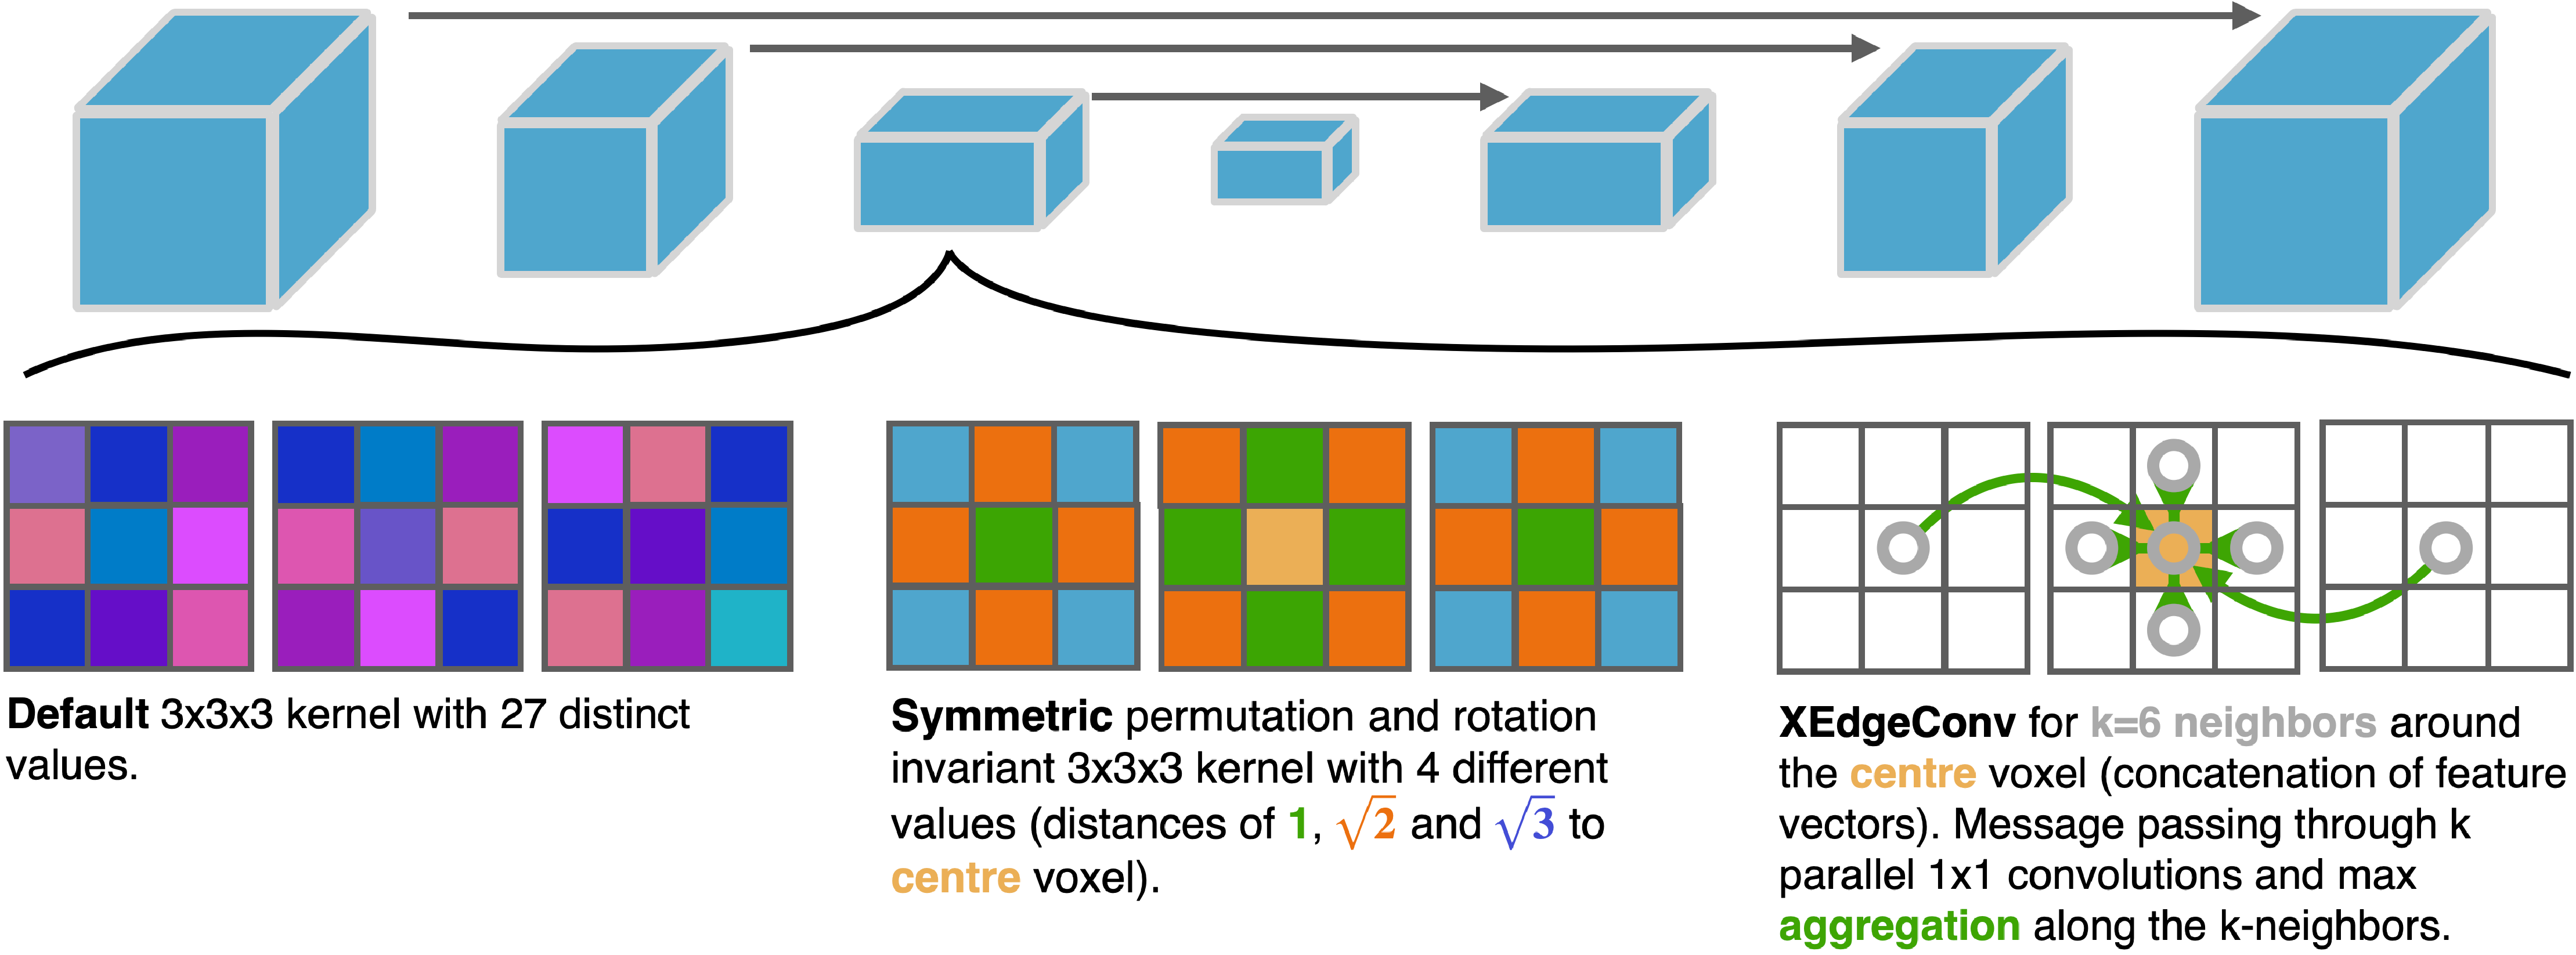
\includegraphics[width=\linewidth]{\xedgeconvPath/figures/geomed2022_figure_xedgemax.pdf}
    \end{figure}
    \paragraph{Symmetric kernels} Our first and most straightforward modified variant of the convolution kernels  uses a reduction of learnable parameters for each filter and channel from 27 to 4 by a rotationally symmetric reflection. To remove any dependency on orientation of the filter kernel, we introduce weight sharing for all elements that have the same distance from the centre. In a $3\times3\times3$ these are four elements with $r=\{0,1,\sqrt{2},\sqrt{3}\}$, see Fig.\,\ref{fig:concept}. This approach is most closely related to diffusion graph CNNs \cite{atwood2016diffusion}, which also learns isotropic graph convolutions that are orientation independent. In a second variant, we experimented with a reflection-only symmetric kernel that comprises 8 distinct elements but found merely small improvements with the downside of losing rotational invariance. Both variants have been studied in SymNets yielding good performance for moderately challenging 2D image classification \cite{dzhezyan2021symmetrical}, but using relatively large kernels and shallow networks.
    Exploring the performance of incorporating such a simplistic concept into state-of-the-art segmentation networks has not been investigated so far and can serve as baseline.

    \paragraph{XEdgeConv kernels} Next, we introduce our proposed \textit{XEdgeConv} operation. In geometric deep learning, the definition of a consistent spatial kernel layout is impossible due to the absence of a regular grid. Hence, the interaction between points (or nodes) in a graph can only depend on point-wise features. The introduction of graph attention \cite{velivckovic2018graph} and edge convolutions \cite{wang2019dynamic} opened the possibility of learning to compute edge attention weights and neural messages respectively that depend on intermediate feature vectors of both considered nodes connected by an edge in the graph. For XEdgeConv a graph that comprises vertices and edges is constructed $\mathcal{G}=(\mathcal{V},\mathcal{E})$, which in the simplest case can be a Euclidean knn-graph. Edge features of two nodes $i$ and $j$ that are in close spatial proximity are defined as $e_{i,j}=h_{\Theta}(x_i,x_j)$, where $x_{i,j}$ are pointwise feature vectors and $h_{\Theta}$ a trainable function. Without loss of generality, we assume $h_{\Theta}$ to be a $1\times1$ convolution of the concatenated feature vectors $x_i$ and $x_j$ with subsequent normalisation and ReLu activation. Once all $k$ messages are computed, a symmetric aggregation is required to combine the information that is received from the neighbourhood. Here we opt for a $\mathrm{max}$ operator\footnote{For irregular graphs the pooling layer would need to be replaced by a graph coarsening layer such as in \cite{qi2017pointnet++}}, which goes along with the standard nnUNet pooling operation, followed by another $1\times1$ convolution, normalisation and nonlinearity, but using averaging yielded similar performance in preliminary experiments. Note, that a na\"{i}ve implementation of $h_{\Theta}$ would require $k$ computations per feature channel. Since, a linear transform after concatenation can be replaced by computing two individual linear transforms independently and adding their respective results this overhead is reduced from $k$ to 2. Because of weight-sharing the same linear part is required repeatedly for all k neighbours for which a node sends out messages, these computations can be reused. When using image data on a grid, two $1\times1$ convolutions and a gather operation along all directions of knn-neighbours followed by the max aggregation can be used to pass messages.



\section{Implementation and Ablations}
    The global U-Net architecture comprises a base number of channels of 24, five downsampling and upsampling steps in the encoder and decoder part respectively with skip connections to pass features of same scale across the bottleneck (or lower branches) and to achieve highly accurate segmentation of anatomies with varying sizes. To ensure permutation invariance the stride of downsampling should be the same in all dimensions and the upsampling cannot contain learnable transposed convolutions, so we opt for trilinear interpolation instead. The whole architecture uses 22 convolution filters of size $3\times3\times3$ with a maximum channel depth of 320, instance normalisation and leaky ReLU activations.

    \vspace{-6pt}\paragraph{Baselines} As an upper heavy-baseline, we train the standard, nnUNet with 27 unique coefficients in each filter element. The model excelled at all tasks of the Medical Segmentation Decathlon \cite{antonelli2021medical} and incorporates extensive augmentation, including mirroring along all axes, together with a robust cost function --- Dice and cross-entropy loss deeply supervised at multiple scales --- and a patch-based training routine. All hyperparameters, design choices and pre-processing steps follow the rule-based concept described in \cite{isensee2021nnu}. As a light-baseline, we implement a 3D version of MobileNetV3 \cite{howard2019searching} with a lite R-ASPP (atrous spatial pyramid pooling) segmentation head (MobileLRASPP). In addition to changing the dimensionality of the kernels from 2D to 3D, we replace batch by instance normalisation and use leaky ReLU activations to account for smaller batch sizes. Since, the network choices for MobileLRASPP are based on larger (2D) images, we increase\footnote{We did not alter the MobileLRASPP layer count despite smaller image size to stick close to the definition of the basis model} the resolution of 3D patches by a factor of 1.5. The network comprises 62 convolutional layers with residual connections in its backbone, efficient depthwise separable convolutions and large dilation kernels with squeeze-excitation in the segmentation head - counting 6.8 million parameters.
    The network is run in the nnUNet environment to ensure comparability.

    \vspace{-6pt}\paragraph{SymPermutation} As our first concept, we implement rotation symmetric and permutation invariant kernels in two variants: (1) A symmetric kernel which contains only 4 trainable values as shown in Fig.\,\ref{fig:concept} (denoted as \emph{SymPermutation (full)}). (2) A symmetric kernel, which only has the center and its six neighbours as trainable parameters resulting in 2 trainable values (denoted as \emph{SymPermutation (6-nbh)}). The latter variant is closer related to our proposed method, as \emph{XEdgeConv} also only includes six neighbours in our experiments.

    \vspace{-6pt}\paragraph{XEdgeConv} Our method replaces each $3\times3\times3$ convolution with two $1\times1$ kernels, a gathering operation in the immediate six-neighbourhood ($k=6$ in the graph) followed by instance normalisation and ReLU with another subsequent  $1\times1$ convolution, normalisation and leaky ReLU. We reduced the base number of feature channels from 24 to 16 and use the arithmetic mean of the number of input and output channels for the specification of the intermediate feature width between two subsequent convolutions.
    We can reduce from 30.8 to only 2.0 million trainable parameters within the nnUNet framework which boosts inference performance and moreover benefits of complete rotation and permutation equivariance.


\section{Experiments and Results}

    Various datasets could have been chosen to evaluate our methodological contribution. We opted for one abdominal CT and a cardiac MRI segmentation dataset:

    \paragraph{Abdomen-CT}
    % The public ``beyond the cranial vault''
    \begin{figure}[t]
        \vspace{-20pt}\caption{Left: Overview of model resource usage and accuracy on abdomen CT experiments. XEdgeConv excels with the smallest number of parameters and FLOPS and second best accuracy. Right: The validation accuracy and standard deviation w.r.t. to the number of training epochs.}
        \label{fig:results}
        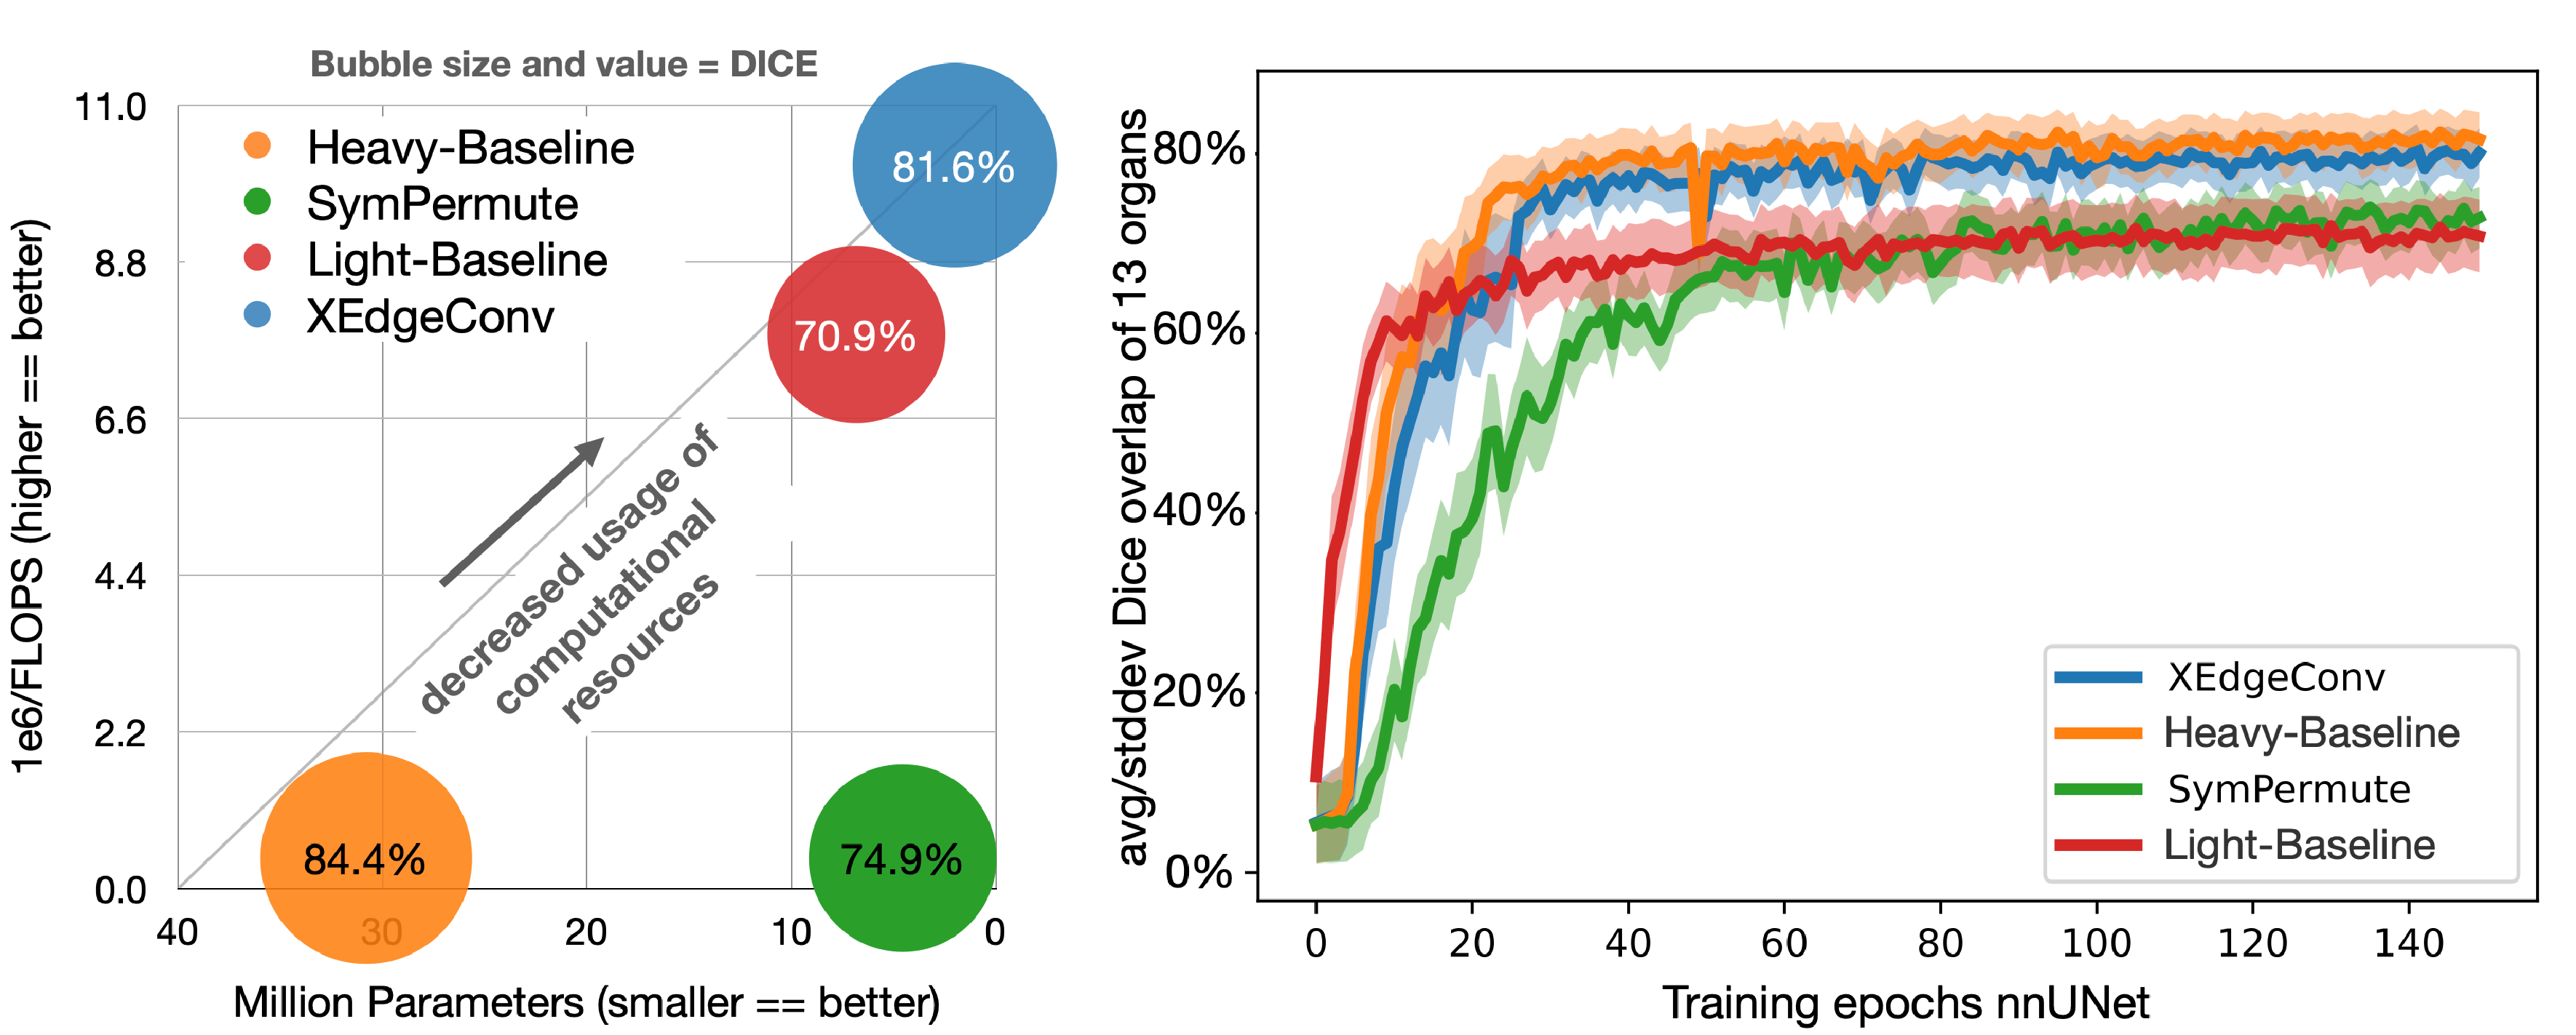
\includegraphics[width=\linewidth]{\xedgeconvPath/figures/geomed2022_figure_xedge_bubble.pdf}
    \end{figure}
    In this task we are using the abdominal CT dataset described in \cite{xu2016evaluation} used in the Learn2Reg 2020 challenge \cite{hering2021learn2reg}. For the latter, a pre-processed version exists that consists of resampling to isotropic resolution of 2mm, automatic cropping to a similar field-of-view and affine pre-registration to a canonical space\footnote{Dataset: \url{https://drive.google.com/uc?export=download&id=1aWyS_mQ5n7X2bTk9etHrn5di2-EZEzyO}}. To give an impression of the variability of organ shapes, we can compute the overlap of copying the segmentation masks from another randomly selected scan resulting in a very low average Dice overlap of 28.1\%.
    We split the data into 20 training and 10 validation scans with 13 anatomical labels each. We train all networks for 150 epochs with default settings. During inference test-time augmentation (TTA) is used only for the two full-kernel variants (heavy- and light-baseline), which boosts their performance by $\approx1\%$point at the cost of 8-times longer inference. We used pytorch 1.10 and either a Nvidia RTX A4000 or A40 (with 16 and 48 GByte VRAM respectively) for training all models. Training each epoch takes 230 secs. for the heavy-baseline, 180 secs. for symmetric permutations, 100 secs. for the light-baseline (MobileLRASPP) and between 290--500 secs. for our proposed model (depending on whether memory checkpointing is employed for reduced VRAM). The CPU inference time of XEdgeConv is 25 times faster than the heavy-baseline (considering TTA) and 3.2 times faster on a single pass.

    Tab.\,\ref{tab:results} (left) highlights the differences across methods and shows that XEdgeConv can drastically reduce the required model capacity and complexity to each state-of-the-art performance.
    This is in contrast to more simplistic symmetric permutation invariant kernels and depth-wise separable convolutions that each result in a substantial drop in quality.
    The detailed numerical results in Tab.\,\ref{tab:results} demonstrates the very accurate results that can be obtained with our model that has 15$\times$ fewer parameters than the baseline across all anatomical structures (with a small exception of the stomach, for which rotational invariance seems to be a disadvantage). Fig.\,\ref{fig:visual} clearly shows the benefit of our model when applied to permuted input data, where the performance of the baseline nnUNet drops to nearly half (45.1\% vs. 84.4\%) but our XEdgeConv method retains its high scores (81.6\% vs. 78.8\%).

    \begin{table}
        \caption{Dice overlap of 10 unseen 3D abdominal CT scans with 9 of 13 structures shown. XEdgeConv (ours) can maintain high scores at a  significantly reduced parameter count. Class labels: Spleen \textcolor{spleen}{$\blacksquare$}, right kidney \textcolor{rkidney}{$\blacksquare$}, left kidney \textcolor{lkidney}{$\blacksquare$}, gallbladder \textcolor{gallbladder}{$\blacksquare$}, esophagus \textcolor{esophagus}{$\blacksquare$}, liver \textcolor{liver}{$\blacksquare$}, stomach \textcolor{stomach}{$\blacksquare$}, aorta \textcolor{aorta}{$\blacksquare$} and pancreas \textcolor{pancreas}{$\blacksquare$}.}
        \label{tab:results}

        \resizebox{\textwidth}{!}{\begin{tabular}{lS[table-format=2.1]r|ccccccccc|cc|ccc}
        \textbf{Method} & \textbf{\#Param.} & \textbf{Input \(\circlearrowleft\)} &\textcolor{spleen}{$\blacksquare$}& \textcolor{rkidney}{$\blacksquare$}& \textcolor{lkidney}{$\blacksquare$}& \textcolor{gallbladder}{$\blacksquare$} & \textcolor{esophagus}{$\blacksquare$} &\textcolor{liver}{$\blacksquare$}&\textcolor{stomach}{$\blacksquare$} & \textcolor{aorta}{$\blacksquare$} & \textcolor{pancreas}{$\blacksquare$}&\textbf{avg.(13)} \\

        \hline
        Light-baseline  & 6.8 M & permuted & 24.2 & 71.2 & 80.0 & 11.3 & 7.0 & 82.7 & 23.8 & 18.1 & 9.4 & 29.5 $\pm$ 9.0\%\\
        Heavy-baseline  & 30.5 M & permuted &61.4&88.0&88.9&41.3&31.0&86.1&56.5&31.0&39.7& 45.1 $\pm$ 8.7\%\\
        SymPermutation (6-nbh)  & 2.0 M & permuted & 80.3 & 86.6 & 87.1 & 46.1 & 30.0 & 86.8 & 54.4 & 71.6 & 43.7 & 59.5 $\pm$ 12.4\%\\
        SymPermutation (full)  & 4.6 M & permuted & 75.1 & 85.5 & 93.1 & 37.8 & 24.9 & 89.9 & 58.3 & 77.1 & 43.1 & 60.2 $\pm$ 12.4\%\\
        SymPermutation (6-nbh)  & 2.0 M & normal & 90.7 & 90.0 & 92.3 & 44.1 & 67.2 & 94.0 & 73.4 & 80.7 & 54.5 & 70.3 $\pm$ 5.8\%\\
        Light-baseline  & 6.8 M & normal &87.6&89.0&90.9&45.8&70.4&84.1&74.3&77.5&64.9& 71.5  $\pm$ 6.0\%\\
        SymPermutation (full)  & 4.6 M & normal &90.3&91.0&93.2&66.2&61.4&94.1&74.7&83.5&58.1& 74.9 $\pm$ 5.9\%\\
        \textbf{XEdgeConv} & 2.0 M & permuted & 93.6&90.8&91.5&58.3&74.2&95.1&78.6&84.3&70.8& \textbf{78.8 $\pm$ 5.0}\%\\
        \textbf{XEdgeConv}  & 2.0 M & normal &94.0&91.8&93.9&77.4&75.1&96.2&79.8&88.2&71.7& \textbf{81.6 $\pm$ 4.0}\%\\
        Heavy-baseline  & 30.5 M & normal&95.2&93.7&93.2&73.3&76.9&96.8&91.1&91.6&76.3& 84.4 $\pm$ 3.2\%\\
        \end{tabular}}
    \end{table}
    \begin{figure}[ht]
        \caption{Prediction on a normally orientated scan (left) and a permuted input (right).
        Our XEdgeConv method maintains performance.
        }
        \label{fig:visual}
        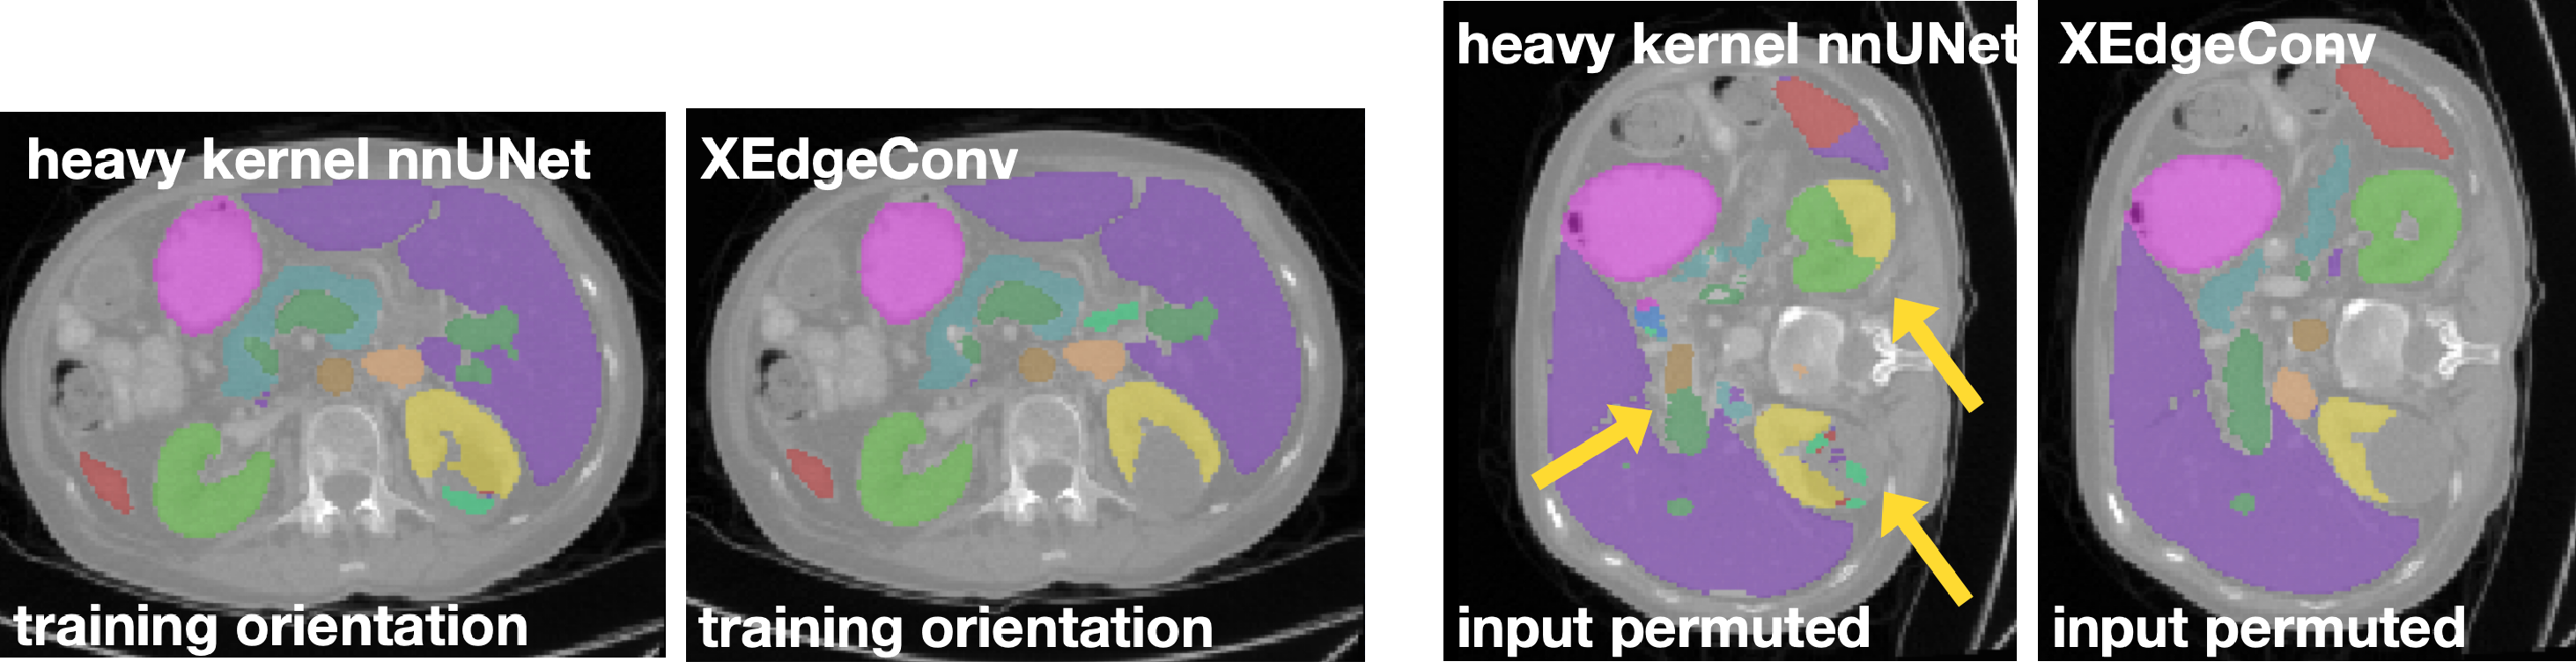
\includegraphics[width=.85\linewidth]{\xedgeconvPath/figures/geomed2022_figure_xedge_visual.pdf}
    \end{figure}

    \paragraph{Cardiac-MRI} As the heart's orientation can vary across patients, we found it suitable to show the influence of rotational and permutational invariant network training. The dataset described in \cite{zhuang2019evaluation} contains MRI scans of the whole heart and seven cardiac labels annotated by experts. Additional to the inter-patient differences in heart orientation, the MRI data subset was acquired in two different canonical scanner directions (6x RIA, 14x AIL)\footnote{Directional convention is defined as: \textbf{R}ight to \textbf{L}eft, \textbf{A}nterior to \textbf{P}osterior, \textbf{S}uperior to \textbf{I}nferior}.
    We split data such that training on AIL samples and testing on RIA samples introduced an additional domain gap to the network. The MRI volumes were resampled at 1.5$\times$1.5$\times$1.5mm and centre-cropped around the ground truth label centroid to a size of 200$\times$200$\times$200 voxels.
    \begin{table}
        \caption{
            Dice overlap of 6 unseen cardiac scans under RIA orientation domain shift (training with AIL orientation). Labels: left myocardium \textcolor{left_myocardium}{$\blacksquare$}, left atrium \textcolor{left_atrium}{$\blacksquare$}, left ventricle \textcolor{left_ventricle}{$\blacksquare$}, right atrium \textcolor{right_atrium}{$\blacksquare$}, right ventricle \textcolor{right_ventricle}{$\blacksquare$}, ascending aorta \textcolor{ascending_aorta}{$\blacksquare$} and pulmonary artery \textcolor{pulmonary_artery}{$\blacksquare$}.
        }
        \label{tab:results_mmwhs}
        \resizebox{\textwidth}{!}{%
            \begin{tabular}{ll|ccccccc|c}

                \textbf{Method}& \textbf{Input \(\circlearrowleft\)}&\textcolor{left_myocardium}{$\blacksquare$}& \textcolor{left_atrium}{$\blacksquare$}& \textcolor{left_ventricle}{$\blacksquare$}& \textcolor{right_atrium}{$\blacksquare$} & \textcolor{right_ventricle}{$\blacksquare$} &\textcolor{ascending_aorta}{$\blacksquare$}&\textcolor{pulmonary_artery}{$\blacksquare$} &\textbf{avg.(7)}\\
                \hline

                Light-baseline  & RIA & 18.0 & 6.2 & 17.6 & 45.7 & 14.4 & 40.2 & 32.5 & 24.9 $\pm$ 14.2\%\\
                Heavy-baseline  & RIA & 25.7 & 16.7 & 26.7 & 39.5 & 3.9 & 52.3 & 31.7 & 28.1 $\pm$ 17.9\% \\
                SymPermutation (6-nbh)  & RIA & 5.8 & 47.1 & 6.7 & 50.5 & 15.9 & 48.4 & 46.3 & 31.5 $\pm$ 18.5\% \\
                SymPermutation (full)  & RIA & 20.6 & 69.2 & 22.3 & 49.4 & 15.0 & 61.2 & 42.4 & 40.0 $\pm$ 18.9\% \\
                \textbf{XEdgeConv} & RIA & 49.7 & 84.9 & 52.1 & 56.9 & 40.3 & 71.2 & 59.7 & \textbf{59.3 $\pm$ 22.1\%}  \\
            \end{tabular}
        }
    \end{table}
    For this setting, we experience a large improvement in Dice mean accuracies, shown in Tab.\,\ref{tab:results_mmwhs}. The visual results of one test case are shown in Fig.\,\ref{fig:visual_mmwhs} for the centre slice and the 3D volume (ground truth, nnUNet full-kernel baseline and XEdgeConv).
    The potential of our method can also be seen in cardiac segmentation where the heavy-baseline nnUNet cannot overcome the orientation domain gap as successful as our method (28.1\% vs. 59.3\%, Tab.\,\ref{tab:results_mmwhs}).

    Test case predictions are more convincing for some classes (e.g. the left atrium and pulmonary artery in Fig.\,\ref{fig:visual_mmwhs}).

    \begin{figure}[h]
        \vspace{-20pt}\caption{Heavy-baseline and XEdgeConv predictions given a RIA oriented test case. Networks were trained on AIL oriented data. With our method more reasonable predictions are achieved (see left atrium and right ventricle prediction, arrow). Class labels see Tab.\,\ref{tab:results_mmwhs}.}
        \label{fig:visual_mmwhs}
        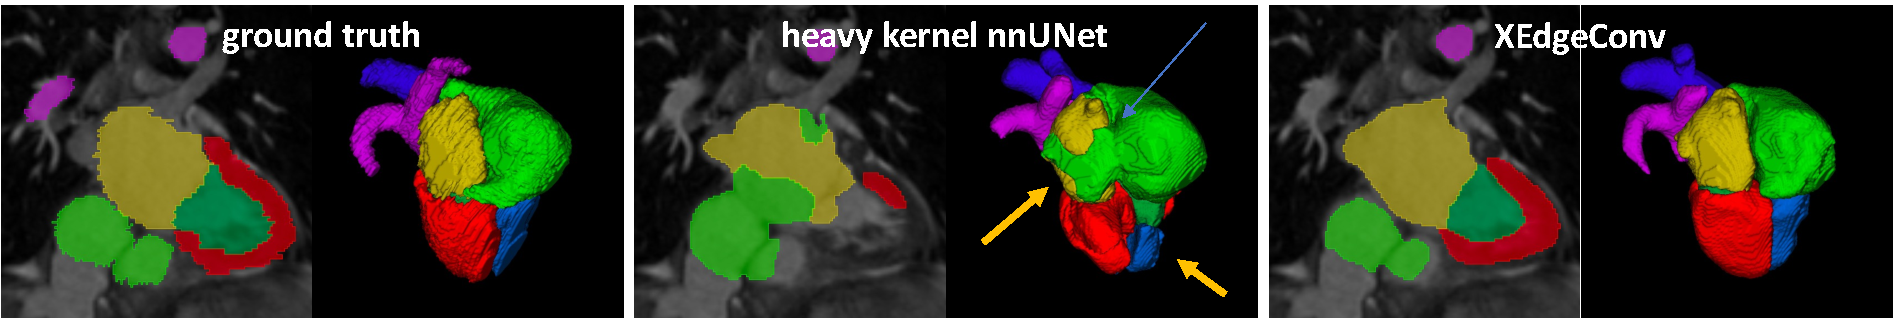
\includegraphics[width=\linewidth]{\xedgeconvPath/figures/mmwhs_overview.pdf}
    \end{figure}



\section{Discussion and Conclusion}
    We have presented a radically new concept for computing spatial convolutions in a 3D segmentation U-Net that does not directly use a spatial filter kernel but is rather based on the concept of neural message passing. This comes at the benefit of rotation, reflection and permutation equivariance. The benefits of using mirror (reflection) augmentations in semantic segmentation had been previously discussed \cite{isensee2021nnu}, but enabling equivariance for input permutations offers further robustness, e.g. for potential incomplete meta-data of imaging data in practical use cases (and removes the need for augmentation).

    We evaluated the benefits of transferring graph-convolutions to grid-data in two medical segmentation tasks. Our XEdgeConv-Net reduces the number of parameters by a factor of 15 (i.e. by 93\%) and the number of computational FLOPS by 95\% compared to the baseline nnUNet model while resulting in a minor reduction of 2.8\% in Dice accuracy (81.6\% vs 84.4\%) for the first experiment (Abdomen-CT), with data that had been canonically aligned as pre-processing. For canonically unaligned data --- such as MRI images acquired with different clinical scanning protocols --- we can show that substantial higher Dice accuracies can be achieved (28.1\% vs. 59.3\%). We can thus show that our proposed XEdgeConv minimises the deterioration of 3D U-Net models in the case of domain-shifts introduced by differences in 3D image orientation.
    Obtaining such a strong performance by replacing full convolution kernels with only 2 trainable coefficients (a 15$\times$ fold decrease in model capacity) is an unexpected and surprising result that can initiate further research into trainable graph-based message passing algorithms for segmentation.
    To the best of our knowledge this is the first method that demonstrates advances in voxelised 3D image analysis using concepts from geometric point-cloud learning.
    For inference on CPU, a substantial speed-up (3.2$\times$ without and 25$\times$ with test-time augmentation) is achieved.
    This clearly demonstrates that the reduction of computational operations of geometric deep learning methods translates into more efficient 3D image analysis when applied in clinical practice. However, due to the highly optimised tensor compute units present in GPU servers, this does not directly translate into faster training times during development.
    In future work, other graph neighbourhoods and message passing schemes could be considered and a more varied set of datasets could be studied to gain further insights into the relevance of different invariances for other applications.
